\documentclass[a4paper, 9pt]{article}          
\usepackage[slovene]{babel}                     
\usepackage[utf8]{inputenc}                    
\usepackage[T1]{fontenc}                        
\usepackage{lmodern} 	                        
\usepackage{amsmath}                           
\usepackage{enumerate}
\usepackage{graphicx}
\usepackage{subfig}
\usepackage{courier}
\usepackage{float}
\usepackage{listings}
\usepackage{hyperref}
\lstset{
  basicstyle=\ttfamily,
  columns=fullflexible,
  breaklines=true,
}
\graphicspath{ {./images/} }
\begin{document}

\begin{titlepage}
    \begin{center}

    \large
    Univerza v Ljubljani\\
        \normalsize
        Fakulteta za matematiko in fiziko\\

    \vspace{5 cm} 

        \large
        Finančni praktikum\\


    \vspace{0.5cm}
    \LARGE
        \textbf{Najdaljša pot v grafu}

    \vspace{0.5 cm}

    \large
        Vid Treven, Val Groleger \\


    \vspace{1.5cm}
    \normalsize
        Mentorja: prof. dr. Sergia Cabello Justo, doc. dr. Janoš Vidali
    \vspace{3cm}


    \vfill

        \large Ljubljana, 2022

    \end{center}
\end{titlepage}

%\tableofcontents
%\pagebreak

\section{Uvod}
Za projektno nalogo pri predmetu finančni praktikum bova iskala najdaljše poti v grafih. Za razliko od problema iskanja najkrajše poti v grafih brez negativnih ciklov, ki je rešljiv v polinomskem času, pa je problem iskanja najdaljše poti NP-težak za splošne grafe. Za usmerjene aciklične grafe poznamo linerni algoritem, ki reši problem, kar je predvsem uporabno pri iskanju kritičnih poti. 

Iskanje Hamiltonove poti v grafu $G$ z $n$ vozlišči lahko reduciramo na iskanje najdaljše poti, saj graf vsebuje Hamiltonovo pot, če je dolžina najdaljše poti grafa $G$ enaka $n-1$. Ker je iskanje Hamiltonove poti v grafu NP-težak problem, je posledično tudi iskanje najdaljše poti v grafu NP-težak problem. Če bi iskanje najdaljše poti bil polinomski problem, bi lahko poiskali najdaljšo pot v grafu in jo primerjali s številom vozlišč. Potemtakem bi bilo iskanje Hamiltonove poti polinomski problem, kar pa vemo, da ni.

Iskala bova najdaljše poti v usmerjenih uteženih in neuteženih grafih. Pri tem se bova pri uteženih grafih omejila na grafe, ki jih je mogoče topološko urediti, saj v tem primeru poznamo učinkovit algoritem. Za neutežene grafe pa se ne bova posebej omejila. Pri tem bova uporabila dva algoritma: 
\begin{itemize}
    \item iskanje v globino (kasneje DFS) in
    \item algoritem, ki temelji na barvanju vozlišč (kasneje barvno kodiranje oziroma color coding).
\end{itemize}

Te algoritme bova napisala v programskem jeziku python in jih tam tudi preizkusila.\\
Za konec bova za omenjene algoritme generirala naključne grafe in na njih uporabila algoritme. Nato bova analizirala računske čase ter primerjala rezultate algoritmov.

\section{Usmerjeni aciklični grafi}
Problem iskanja najdaljše poti v usmerjenih acikličnih grafih smo deloma spoznali že pri predmetu operacijske raziskave. Tam smo iskali najkrajšo pot med dvema vozliščema. Če hočemo poiskati najdaljšo pot, moramo graf $G$ spremeniti tako, da za uteži novega grafa $-G$ vzamemo nasprotne vrednosti utezi grafa $G$. Nato na danem grafu $-G$ poiščemo najkrajšo pot med danima dvema vozliščema. Najdaljša pot med tema dvema vozliščema v grafu $G$ je enaka nasprotni vrednosti najkrajše poti med tema dvema vozliščema v grafu $-G$. Problem iskanja najkrajše poti v danem usmerjenem acikličnem grafu sva reševala s pomočjo topoloske ureditve tega grafa, saj velja, da lahko vsak usmerjeni aciklični graf tudi topološko uredimo. Če so uteži na povezavah nenegativne, potem bo najdaljša pot v grafu zagotovo pot med prvim in zadnjim vozliščem v topološki ureditvi. V simulaciji sva za ta primer generirala take topološke grafe, ki imajo zgolj en začetek in en konec, tako da je res najdaljša pot v grafu enaka najdaljši poti med prvim in zadnjim vozliščem. Seveda morajo biti uteži na povezavah nenegativne. V primeru, ko pa so uteži na povezavah tudi negativne pa najdaljša pot v grafu ni nujno enaka najdaljši poti med začetnim in končnim vozliščem.

\section{Splošni graf}
Kot sva že omenila, je problem iskanja najdaljše poti v splošnem grafu NP-težak oziroma ni polinomski problem. Za splošne grafe bova uporabila dva algoritma DFS in color coding, nato pa bova generirala naključne grafe in ju podrobneje analizirala.

\subsection{Iskanje v globino}
Iskanje v globino je algoritem, ki kot argumente sprejme graf $G = (V,E)$, njegovo vozlišče $v$ in seznama "obiskana" in "pot", ki vsebujeta že obiskana vozlišča oziroma vozlišča v poti. Najprej doda vozlišče $v$ v seznam "obiskana" nato pa generira prazen slovar "poti". Potem preveri vse sosede vozlišča $v$, torej takšna vozlišča, da je $uv \in E$. Pri prvem vozlišču $u$, ki še ni vsebovan v seznamu "obiskana", poveča seznam "pot", tako da mu doda vozlišče $u$. To pot doda v seznam "poti" in na vozlšču $u$ ponovno kliče algoritem, pri čemer je seznam "obisakana" tak, da ima dodano vozlišče $v$, seznam "pot" pa vsebuje še vozlišče $u$. Ta postopek algoritem ponavlja, dokler ne pride do vozlišča, ki nima sosedov, ki še niso bili obiskani. Zatem se vrne do začetnega vozlišča $v$ in postopek ponovi na sosedih, ki še niso bili obiskani.
Koda v pythonu se glasi:

\begin{lstlisting}[language=Python]
    DFS(G,v,obiskana=None, pot=None):
    if obiskana == None:
        obiskana = []
    if pot == None:
        pot = [v]
    obiskana.append(v)
    poti = []
    for vozlisce in G[v]:
        if vozlisce not in obiskana:
            vozlisce_poti = pot + [vozlisce]
            poti.append(tuple(vozlisce_poti))
            poti.extend(DFS(G, vozlisce, obiskana[:], vozlisce_poti))
    return poti
\end{lstlisting}

Algoritem je uporaben, saj lahko z njegovo pomočjo najdemo topološko ureditev in povezane komponente. Vendar pa ima tudi slabosti:
\begin{itemize}
    \item ni nujno, da algoritem vrne pravo rešitev, saj ne pregleda vseh poti,
    \item lahko ima veliko časovno zahtevnost ter še druge slabosti.
\end{itemize}

Za uporabo v najin namen sva funkcijo klicala na vseh vozliščih $v$ generiranega grafa $G$ in poti shranjevala v seznamu poti. Nato sva izračunala najdaljšo pot grafa kot najdaljšo pot v seznamu poti, ki jih je funkcija vračala.

\subsection{Barvno kodiranje}

Naslovni algoritem je aproksimativen algoritem, torej ne vrne točne vrednosti in je točen le z neko verjetnostjo. Vendar se ob ponavljanju algoritma verjetnost njegove pravilnosti poveča.

Ideja barvnega kodiranja je, da vsako vozlišče danega grafa naključno pobarvamo z eno od $k$ barvami. Nato pa poiščemo pot v danem grafu dolžine k, pri katerem je vsako vozlišče različne barve. Verjetnost pravilnosti algoritma ob eni ponovitvi je navzdol omejena z  $e^{-k}$, vendar se ta, kot sem že povedal, z več ponovitvami poveča. Tako lahko z določeno verjetnostjo trdimo, da smo v danem grafu našli ustrezno pot dolžine $k$. V primeru, ko število barv $k$ povečujemo, pa lahko najdemo tudi najdaljšo pot v danem grafu, saj ko bo $k$ večji od dolžine največje poti, ne bomo uspeli najti poti dolžine $k$.

Najprej naključno pobarvamo vozlišča grafa s $k$ barvami. Namesto posameznih barv uporabimo številke $1, 2, 3 \cdots k$. Tako rabimo preveriti, če obstaja pot $1 - 2 - \cdots - k$. Tako lahko odstranimo vse poti, ki ne povezujejo vozlišči pobarvani $i \text{ in } i+1$.

Algoritem lahko izboljšamo, če namesto poti $1 - 2 - \cdots - k$ iščemo pot, v kateri so vse barve vsebovane natanko enkrat. To lahko storimo z dinamičnim programiranjem. Barvna pot je pot po vozliščih grafa, kjer ima vsako vozlišče različno barvo. Nastavimo robni pogoj: $$x(v,i) == \text{TRUE},$$ če obstaja barvna pot, ki se zaključi v vozlišču $v$, ki je obarvano $i$. Nato za vsako podmnožico $C$ barvanja $k$ in vsako vozlišče $v$ grafa $G$ definiramo rekurzivne formule:
$$x(v, C) = \lor _{u \in sosedi(v)} x(u, C \setminus \{ i\} ),$$ kjer je $i$ barvanje vozlišča $v$.
Torej obstaja barvna pot do vozlišča $v$, kadar obstaja vsaj ena barvna pot do sosednjih vozlišč, ki ne vsebuje barve vozlišča $v$. Tako lahko vidimo, da obstaja barvna pot dolžine $k$ v grafu $G$, če je $x(v,{1, 2 \cdots k}) == \text{TRUE}$ za vsaj eno vozlišče $v$ grafa $G$. V tem primeru obstaja v dane grafu pot dolžine $k$. Kot sem že omenil s povečevanje $k$ in večimi ponovitvami barvanj lahko najdemo najdaljšo pot v danem grafu.
Koda algoritma v programskem jeziku Python:
\begin{lstlisting}[language = Python]
    def color_coding(G,K,n = 100): 
    odgovor = 0
    for k in range(2,K+1):
        j = 0
        while j < n:
            j +=1  
            barvanje = {}
            for v in G:
                barvanje[v] = random.randint(1,k)
            x = {}
            mnozice = [frozenset({j for j in range(1, k+1) if (i >> (j-1)) & 1 == 1}) for i in range(2**k)]
            mnozice = sorted([s for s in mnozice if len(s) > 1], key=len)
            for v in G:
                for i in range(1,k+1):
                    x[v,frozenset({i})] = barvanje[v] == i
            for C in mnozice:
                for v in G:
                    b = barvanje[v]
                    x[v, C] = b in C and any(x[u, C - {b}] for u in G[v])
            if any(x[v,mnozice[-1]] for v in G):
                odgovor = k
    return odgovor
\end{lstlisting}
\pagebreak
\section{Simulacija}

\subsection{Generiranje podatkov}
Za namen simulacije sva napisala funkciji, ki generirata naključne usmerejene grafe. Prva funkcija generira utežene grafe pri izbiri števila vozlišč in zgornje ter spodnje meje za uteži povezav. Graf je predstavljen kot slovar vozlišč. Vsako vozlišče ima še en slovar; ključ slovarja je vozlišče, do katerega gre povezava, vrednost pa je utež na tej povezavi. Vsako vozlišče ima povezavo v naslednje vozlišče zagotovljeno (zaradi topološke ureditve), v preostala vozlišča pa se povezave generirajo naključno. Zadnje vozlišče ima povezavo tudi v še eno dodatno vozlišče, kar pa ni ustrezno. A ta napaka nikjer ne zmoti simulacije, zato je ni potrebno odstraniti. Druga funkcija pa generira naključne grafe pri izbiri števila vozlišč. Graf je podan kot slovar, katerega ključi so vozlišča, vrednosti pa so seznami sosedov. Funkcija sosede generirana naključno. Tako so grafi na katerih sva izvajala simulacije medseboj različni.

\subsection{Usmerjeni aciklični grafi}
Pri usmerjenih acikličnih grafih, ki imajo topološko gledano en začetek in en konec s pozitivnimi utežmi na povezavah, sva merila čas, ki ga algoritem \textit{najdaljsa pot} povprečno porabi za eno povezavo v odvisnosti od števila vozlišč in pa v odvisnosti od razpona uteži na povezavi. \\
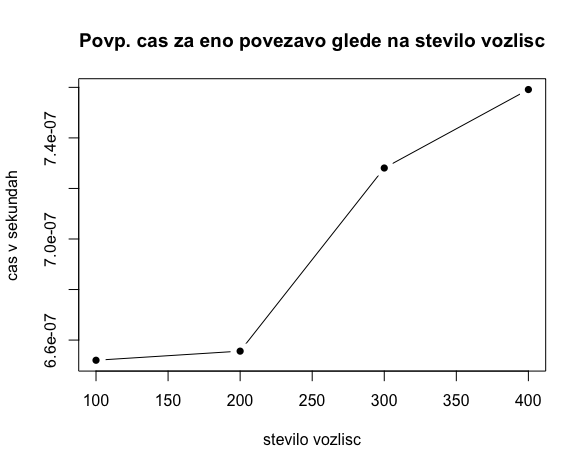
\includegraphics[width = 12cm, height=8cm]{plot_v2.png}\\
Po pričakovanjih, je za eno povezavo potrebno zelo malo časa. Ko večamo število vozlišč se sicer čas povečuje, a so razlike zelo majhne. Podobno se zgodi tudi ko spreminjamo razpon uteži na povezavah, le da tokrat čas varira, ne zgolj narašča.\\
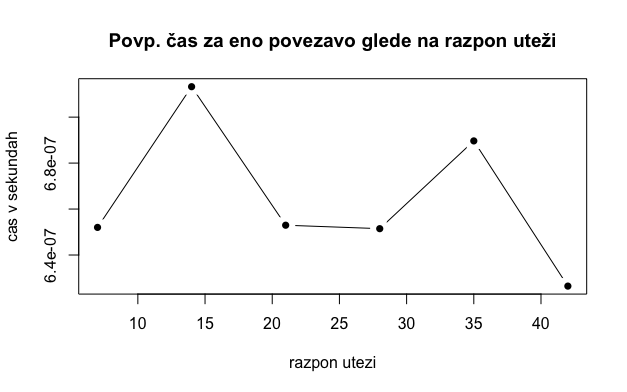
\includegraphics[width = 10cm, height = 6cm]{Rplot.png}


\subsection{Neuteženi grafi}
Pri neuteženih grafih sva sprva preizkušala hitrost algoritma \textit{color coding} v odvisnosti od števila ponovitev na danem grafu. V ta namen sva generirala graf z 8 vozlišči na katerem sva večkrat pognala program, pri tem pa sva vedno barvala graf z enajstimi barvami oziroma sva povečevala število barv do 11. V vsakem poskusu sva iterativno povečala število ponovitev vsakega barvanja po 20. Začela sva z 1 ponovitvijo in zaključila z 981 ponovitvami. Rezultate vidimo na spodnjem grafu. \\
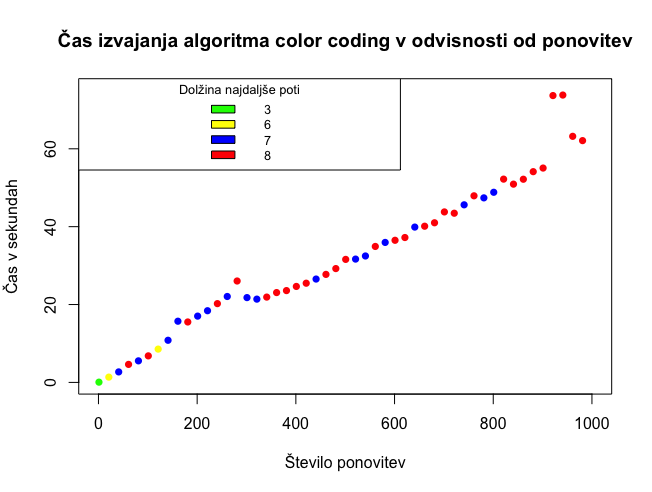
\includegraphics[width = 12cm, height = 8cm]{izvajanje_od_ponovitev.png}\\
Opazimo, da je pri manjšem število ponovitev dolžina najdaljšega zaporedja, ki ga vrne funkcija občutno manjše, kot pri na primer več kot 800. poskusu. Hkrati lahko vidimo, da časovna zahtevnost narašča linearno z večanjem števila ponovitev. 
Nato sva še primerjala hitrost programa \textit{color coding} s hitrostjo programa \textit{DFS}. Za vsako število vozlišč od 5 do 13 sva generirala 15 grafov in na njih za vsako barvo do $K$ ($K$ sva spreminjala za vsako število vozlišč) izvedla 20 ponovitev barvanj nato pa še iskanje v globino. V ta namen sva pripravila dva grafa. Prvi graf prikazuje povprečen čas računanja algoritmov \textit{color coding} in \textit{DFS} za vsako število vozlišč. \\
\includegraphics[width = 12cm, height = 8cm]{povprečen čas.png}\\
Iz grafa lahko razberemo, da se časovna zahtevnost obeh algoritmov s številom vozlišč v proučevanih grafih povečuje. Pri algoritmu \textit{color coding} pa je hitrost povečevanja občutno večja. Meniva, da je razlog za to število ponovitev vsakega barvanja, tako pa se število operacij občutno poveča. Pri proučevanih algoritmih vidimo eksponentno rast potrebnega časa za izračun vrednosti.
Podobne rezultate pa vidimo tudi na drugem grafu, ki prikazuje povprečen čas izvajanja algoritma na povezavo glede na število vozlišč. \\
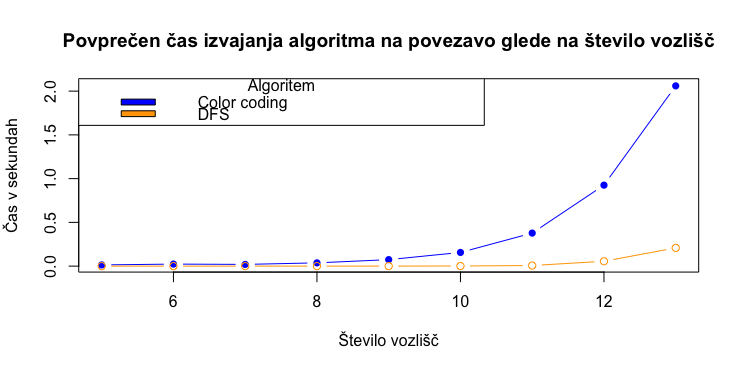
\includegraphics[width = 12cm, height = 9cm]{sim.png}\\
Na drugem grafu opazimo, da se čas izvajanja algoritma na povezavo prav tako povečuje s številom vozlišč grafa. \\
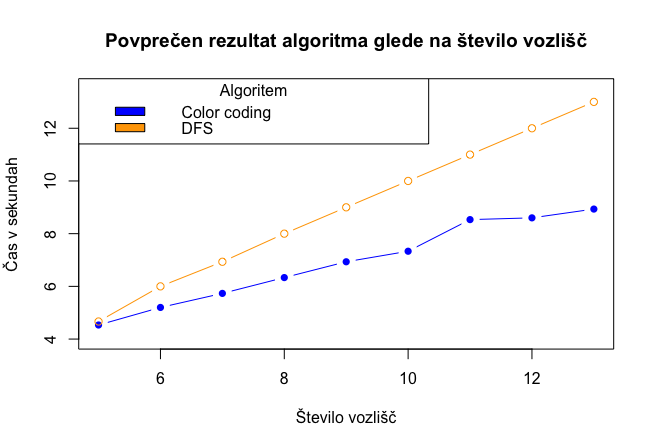
\includegraphics[width =12cm, height = 8cm]{povprecje_pot.png}\\
Na zgornejm grafu lahko vidimo primerjavo povprečnih vrednosti, ki sta jih funkciji vračali pri posameznih številih vozlišč proučevanih grafov. Opazimo, da je povprečje najdaljša poti, ki jo je izračunal algoritem \textit{DFS} večje. Po najnem mnenju je krivec za to aproksimativnost algoritma \textit{color coding}.
Natančnejše rezultate simulacije so dostopne v CSV datotekah objavljenih na repozitoriju na GitHubu.

\section{Viri}
\begin{enumerate}
    \item Zapiski iz predmeta operacijske raziskave, poletni semester 2022, dostopal v novembru in decembru 2022, osebna last.
    \item \href{https://en.wikipedia.org/wiki/Longest \_ path \_ problem}{https://en.wikipedia.org/wiki/Longest \_ path \_ problem}, dostopal v novembru, decembru 2022.
    \item \href{https://en.wikipedia.org/wiki/Color-coding} {https://en.wikipedia.org/wiki/Color-coding}, dostopal v novembru, decembru 2022.
    \item Marx, D. Recent Adventages in FPT and Exact Algorithms for NP-Complete problems. 1. 9. 2015. Dostopno na: \href{http://cs.bme.hu/~dmarx/papers/marx-simons1.pdf} {http://cs.bme.hu/~dmarx/papers/marx-simons1.pdf} [6.12.2022].
\end{enumerate}

\end{document}